\documentclass[10pt, english, aspectratio=169]{beamer}
	\usepackage{geometry}
                \geometry{
                        tmargin=10mm,
                        bmargin=10mm,
                        lmargin=10mm,
                        rmargin=10mm,
                }

	\usetheme{CambridgeUS}

	\usepackage{titlesec}
                \titleformat{\section}
                        {\normalfont\fontsize{16}{16}\bfseries}{\thesection}{0.5em}{}
                \titleformat{\subsection}
                        {\normalfont\fontsize{14}{16}\bfseries}{\thesubsection}{1em}{}
                \titleformat{\subsubsection}
                        {\normalfont\fontsize{11}{16}\bfseries}{\thesubsubsection}{1em}{}

	\usepackage{float}

	\usepackage{longtable}
        \usepackage{multirow}

	\usepackage{caption}
                \captionsetup[table]{labelfont=bf,textfont=bf,font=small,skip=8pt}
                \captionsetup[figure]{labelfont=bf,textfont=bf,font=small,skip=8pt}
        \usepackage{subcaption}
                \captionsetup[subtable]{labelfont=rm,textfont=rm,font=small,skip=8pt,labelformat=parens,labelsep=space}
                \captionsetup[subfigure]{labelfont=rm,textfont=rm,font=small,skip=8pt,labelformat=parens,labelsep=space}

	\renewcommand{\thetable}
                {\thesection.\arabic{table}}                                                         
	\renewcommand{\thesubtable}
                {\roman{subtable}}

	\renewcommand{\thefigure}
                {\thesection.\arabic{figure}}
        \renewcommand{\thesubfigure}
                {\roman{subfigure}}

        \usepackage{hyperref}
                \hypersetup{
                        colorlinks=true,
                        linkcolor=black,
                        filecolor=magenta,
                        urlcolor=cyan,
                        }

        \setlength{\parindent}{0pt}
        \renewcommand{\baselinestretch}{1.25}
        \usepackage{setspace}

        \usepackage{amsmath}
        \usepackage{amssymb}

	\usepackage{graphicx}

	\usepackage{tikz}
                \usetikzlibrary{trees,arrows,topaths}

	\usepackage[utf8]{inputenc}
	\usepackage[T1]{fontenc}

\begin{document}

\pagenumbering{gobble}

	\title{\textsc{CS993 Software Engineering\\ Coursework Assignment}}
	\author{\textsc{Group 2}}
	\date{\textsc{Academic Year 2021/2022}}
        \maketitle

\newpage

\pagenumbering{arabic}

\section{Context}

	\subsection{Specification}

	\begin{itemize}
	\setlength\itemsep{0cm}
		\item Cinema booking system
		\item Three user types: admin, staff, booker 
		\item User interface: HTML, CSS, JavaScript (no bloated IDEs or froymeworks)
		\item Rear-end: SQL (PHPMyAdmin), Python
	\end{itemize}
	
	\begin{center}
	\begin{tabular}{cccc}
		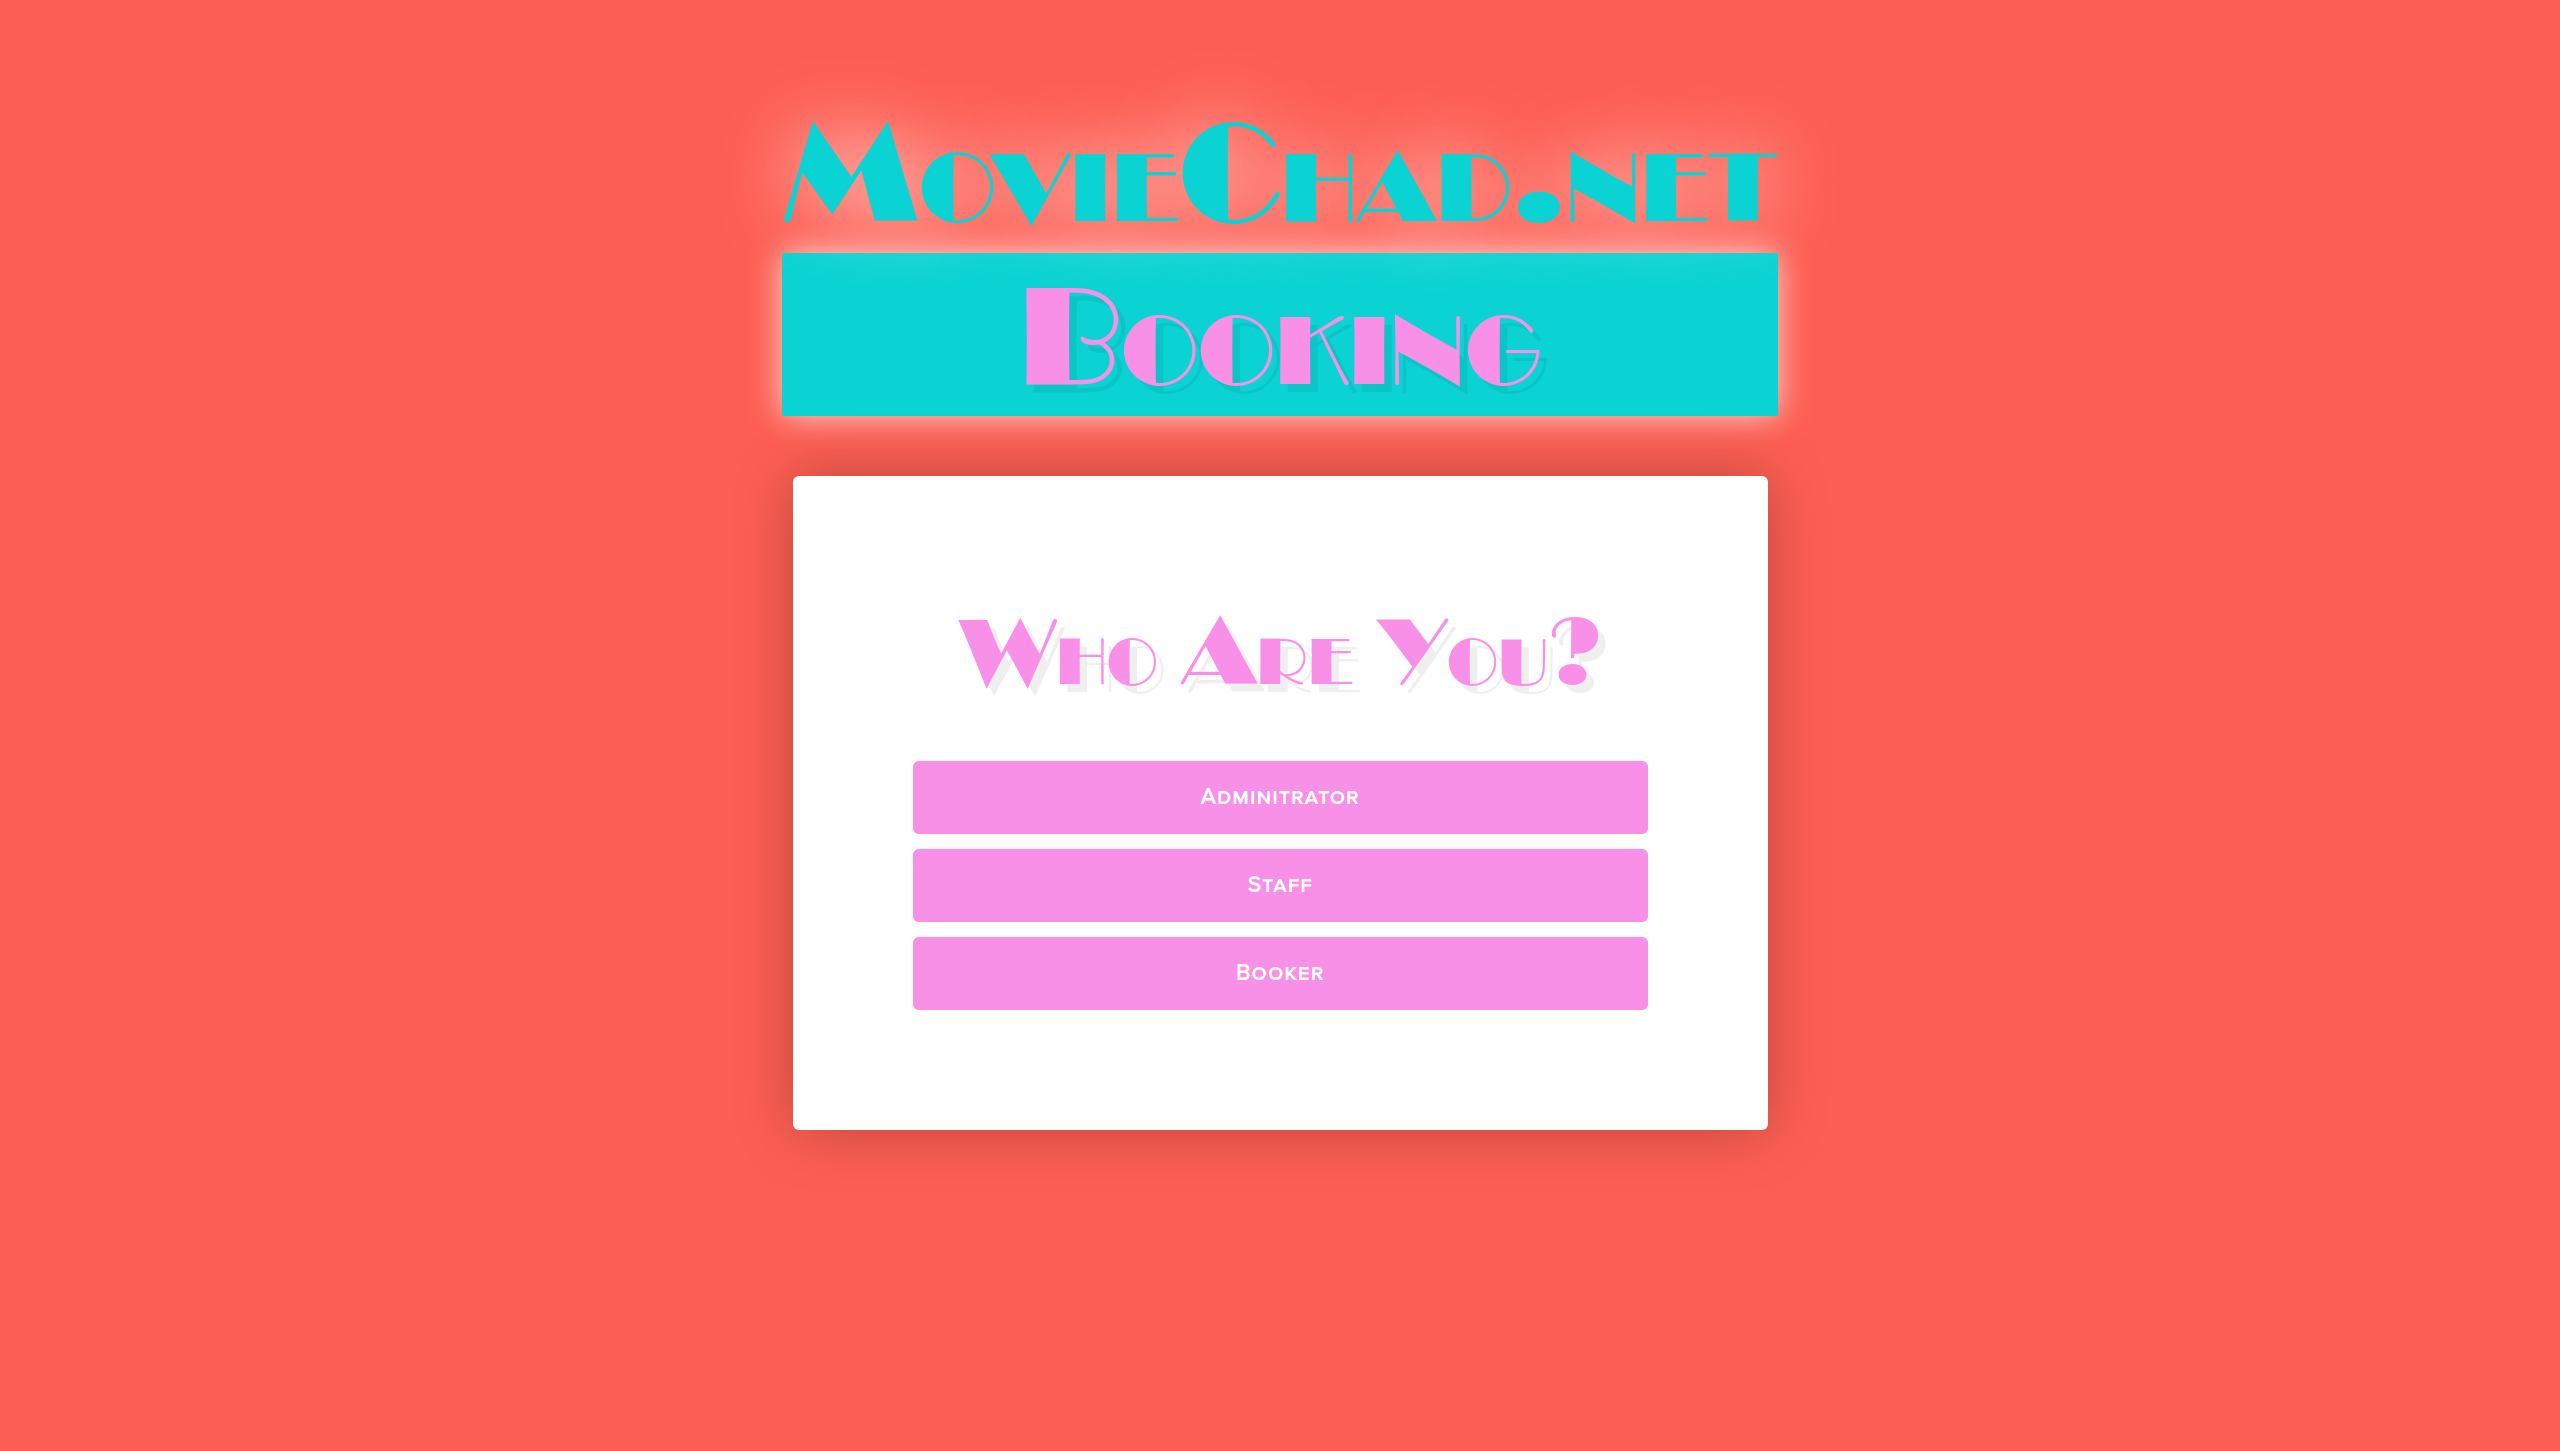
\includegraphics[width=3.25cm,height=2cm]{login.png} & 
		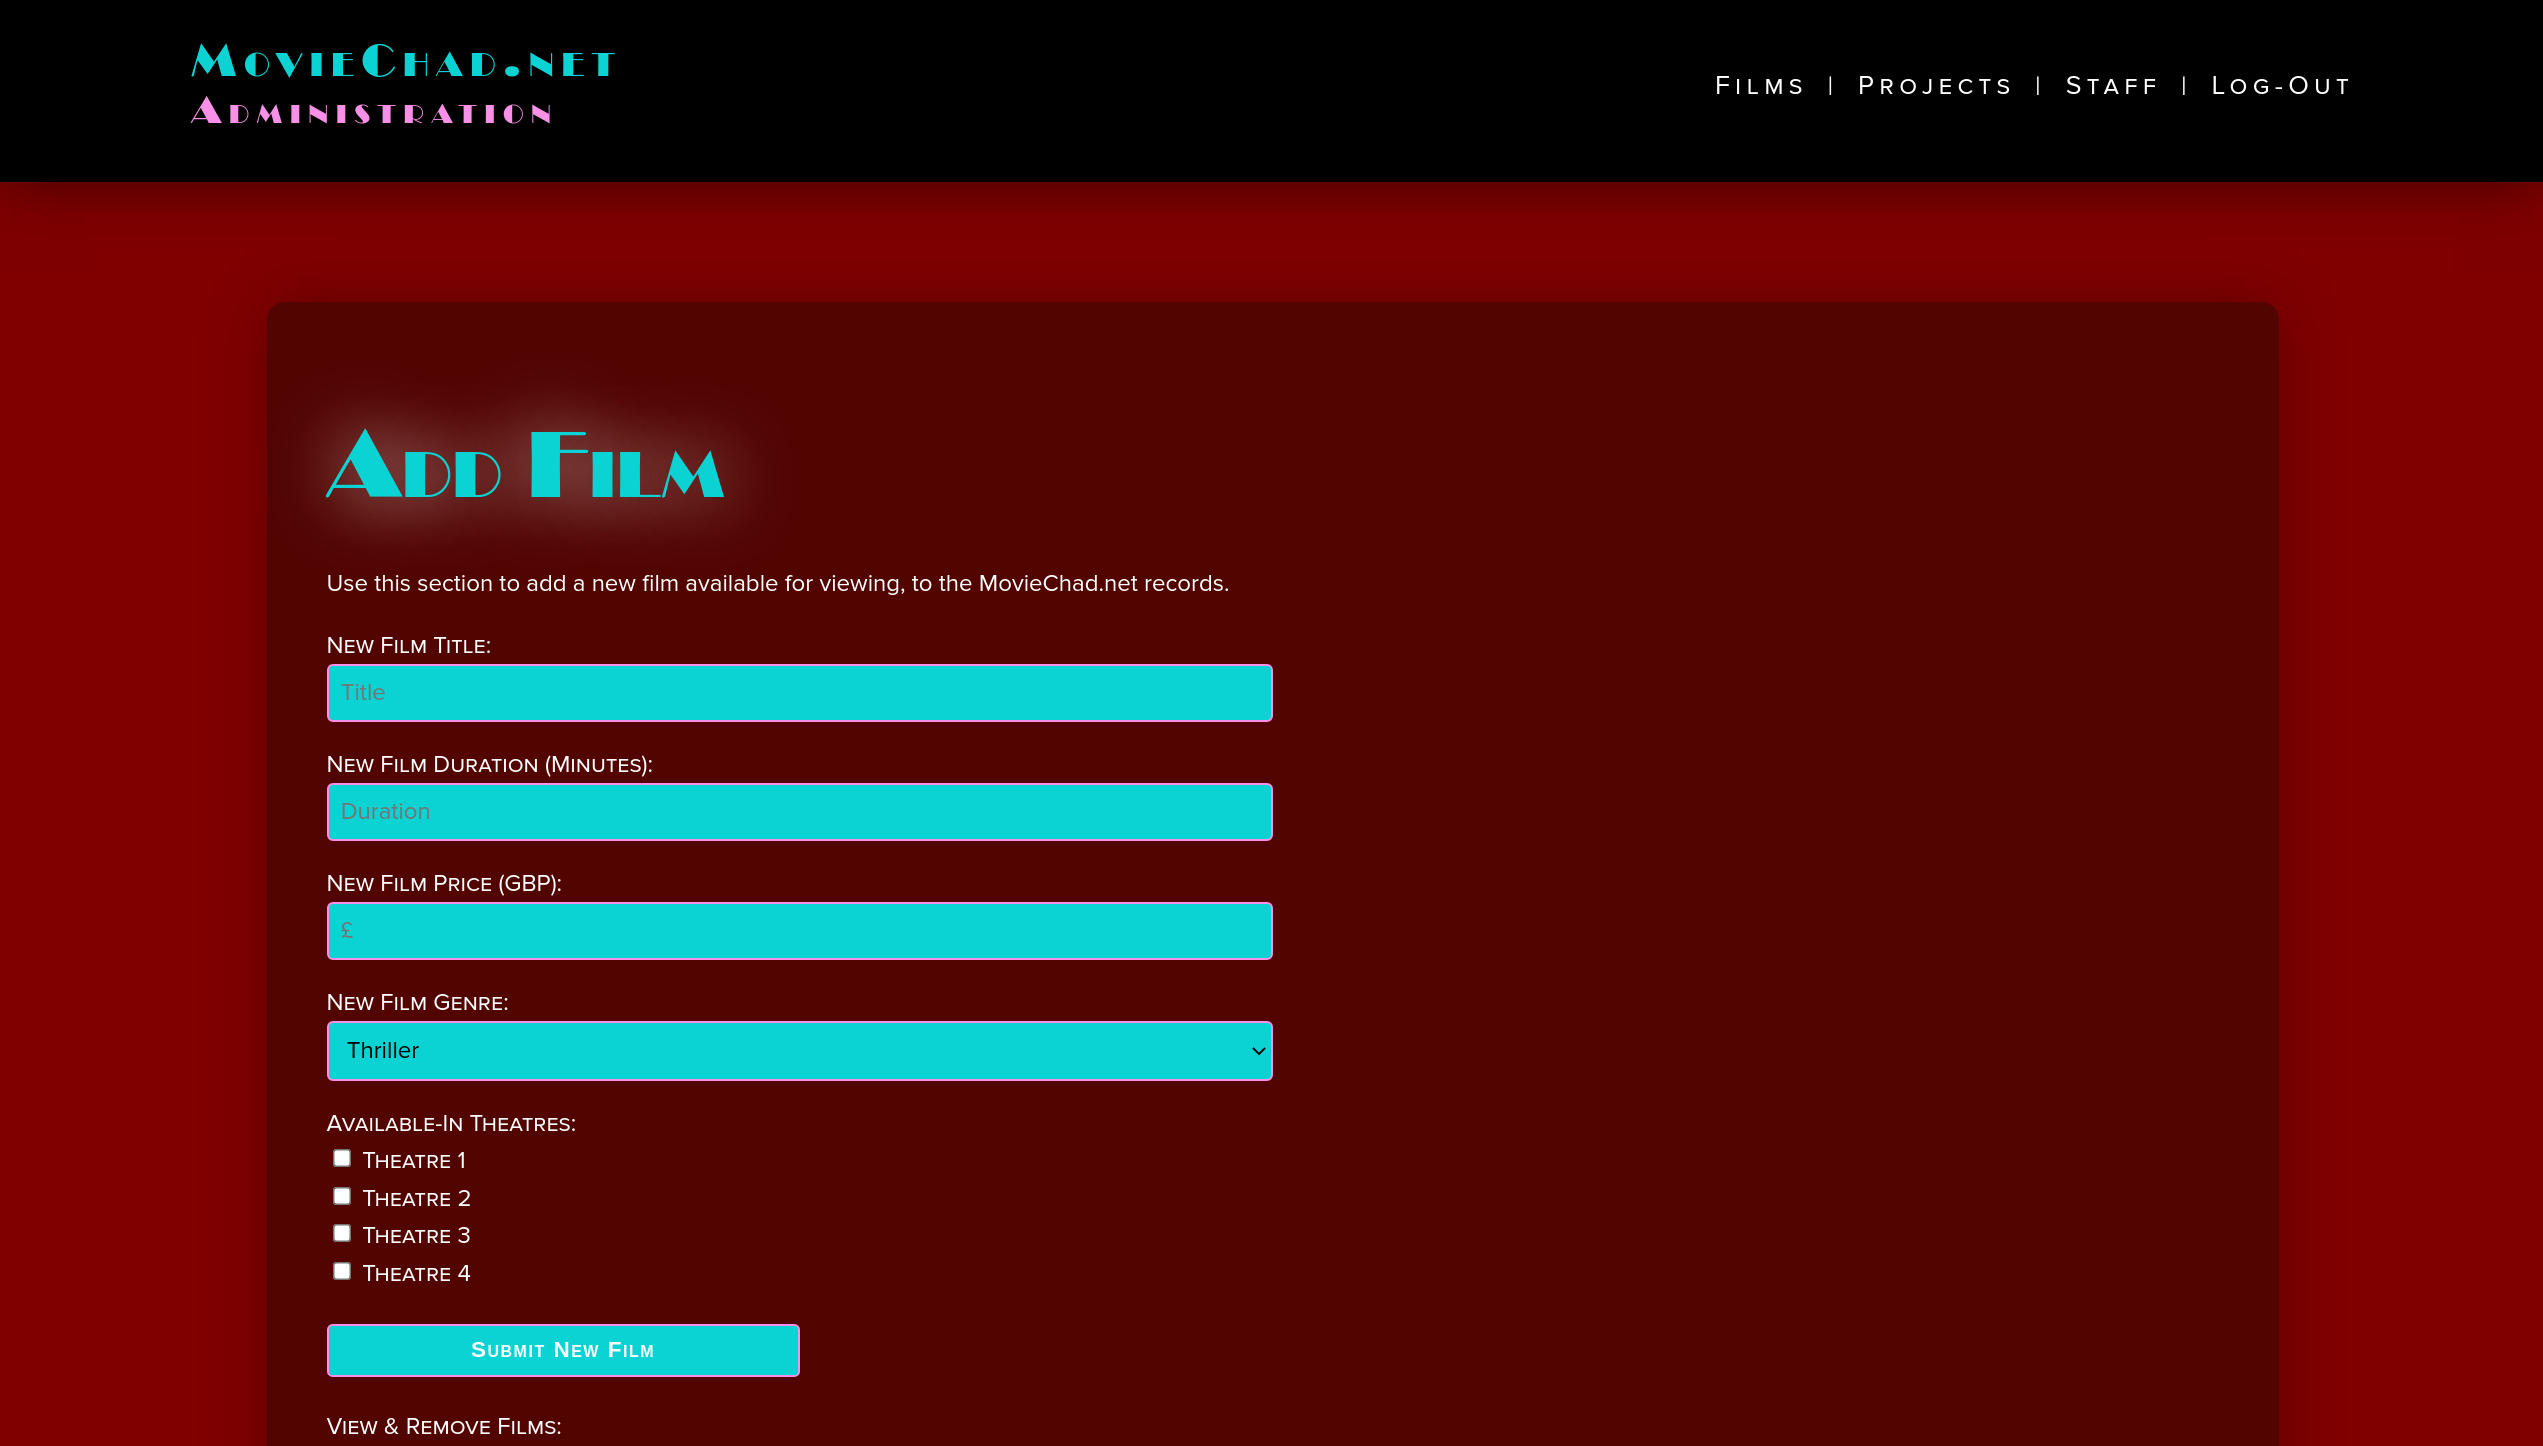
\includegraphics[width=3.25cm,height=2cm]{admin.png} & 
		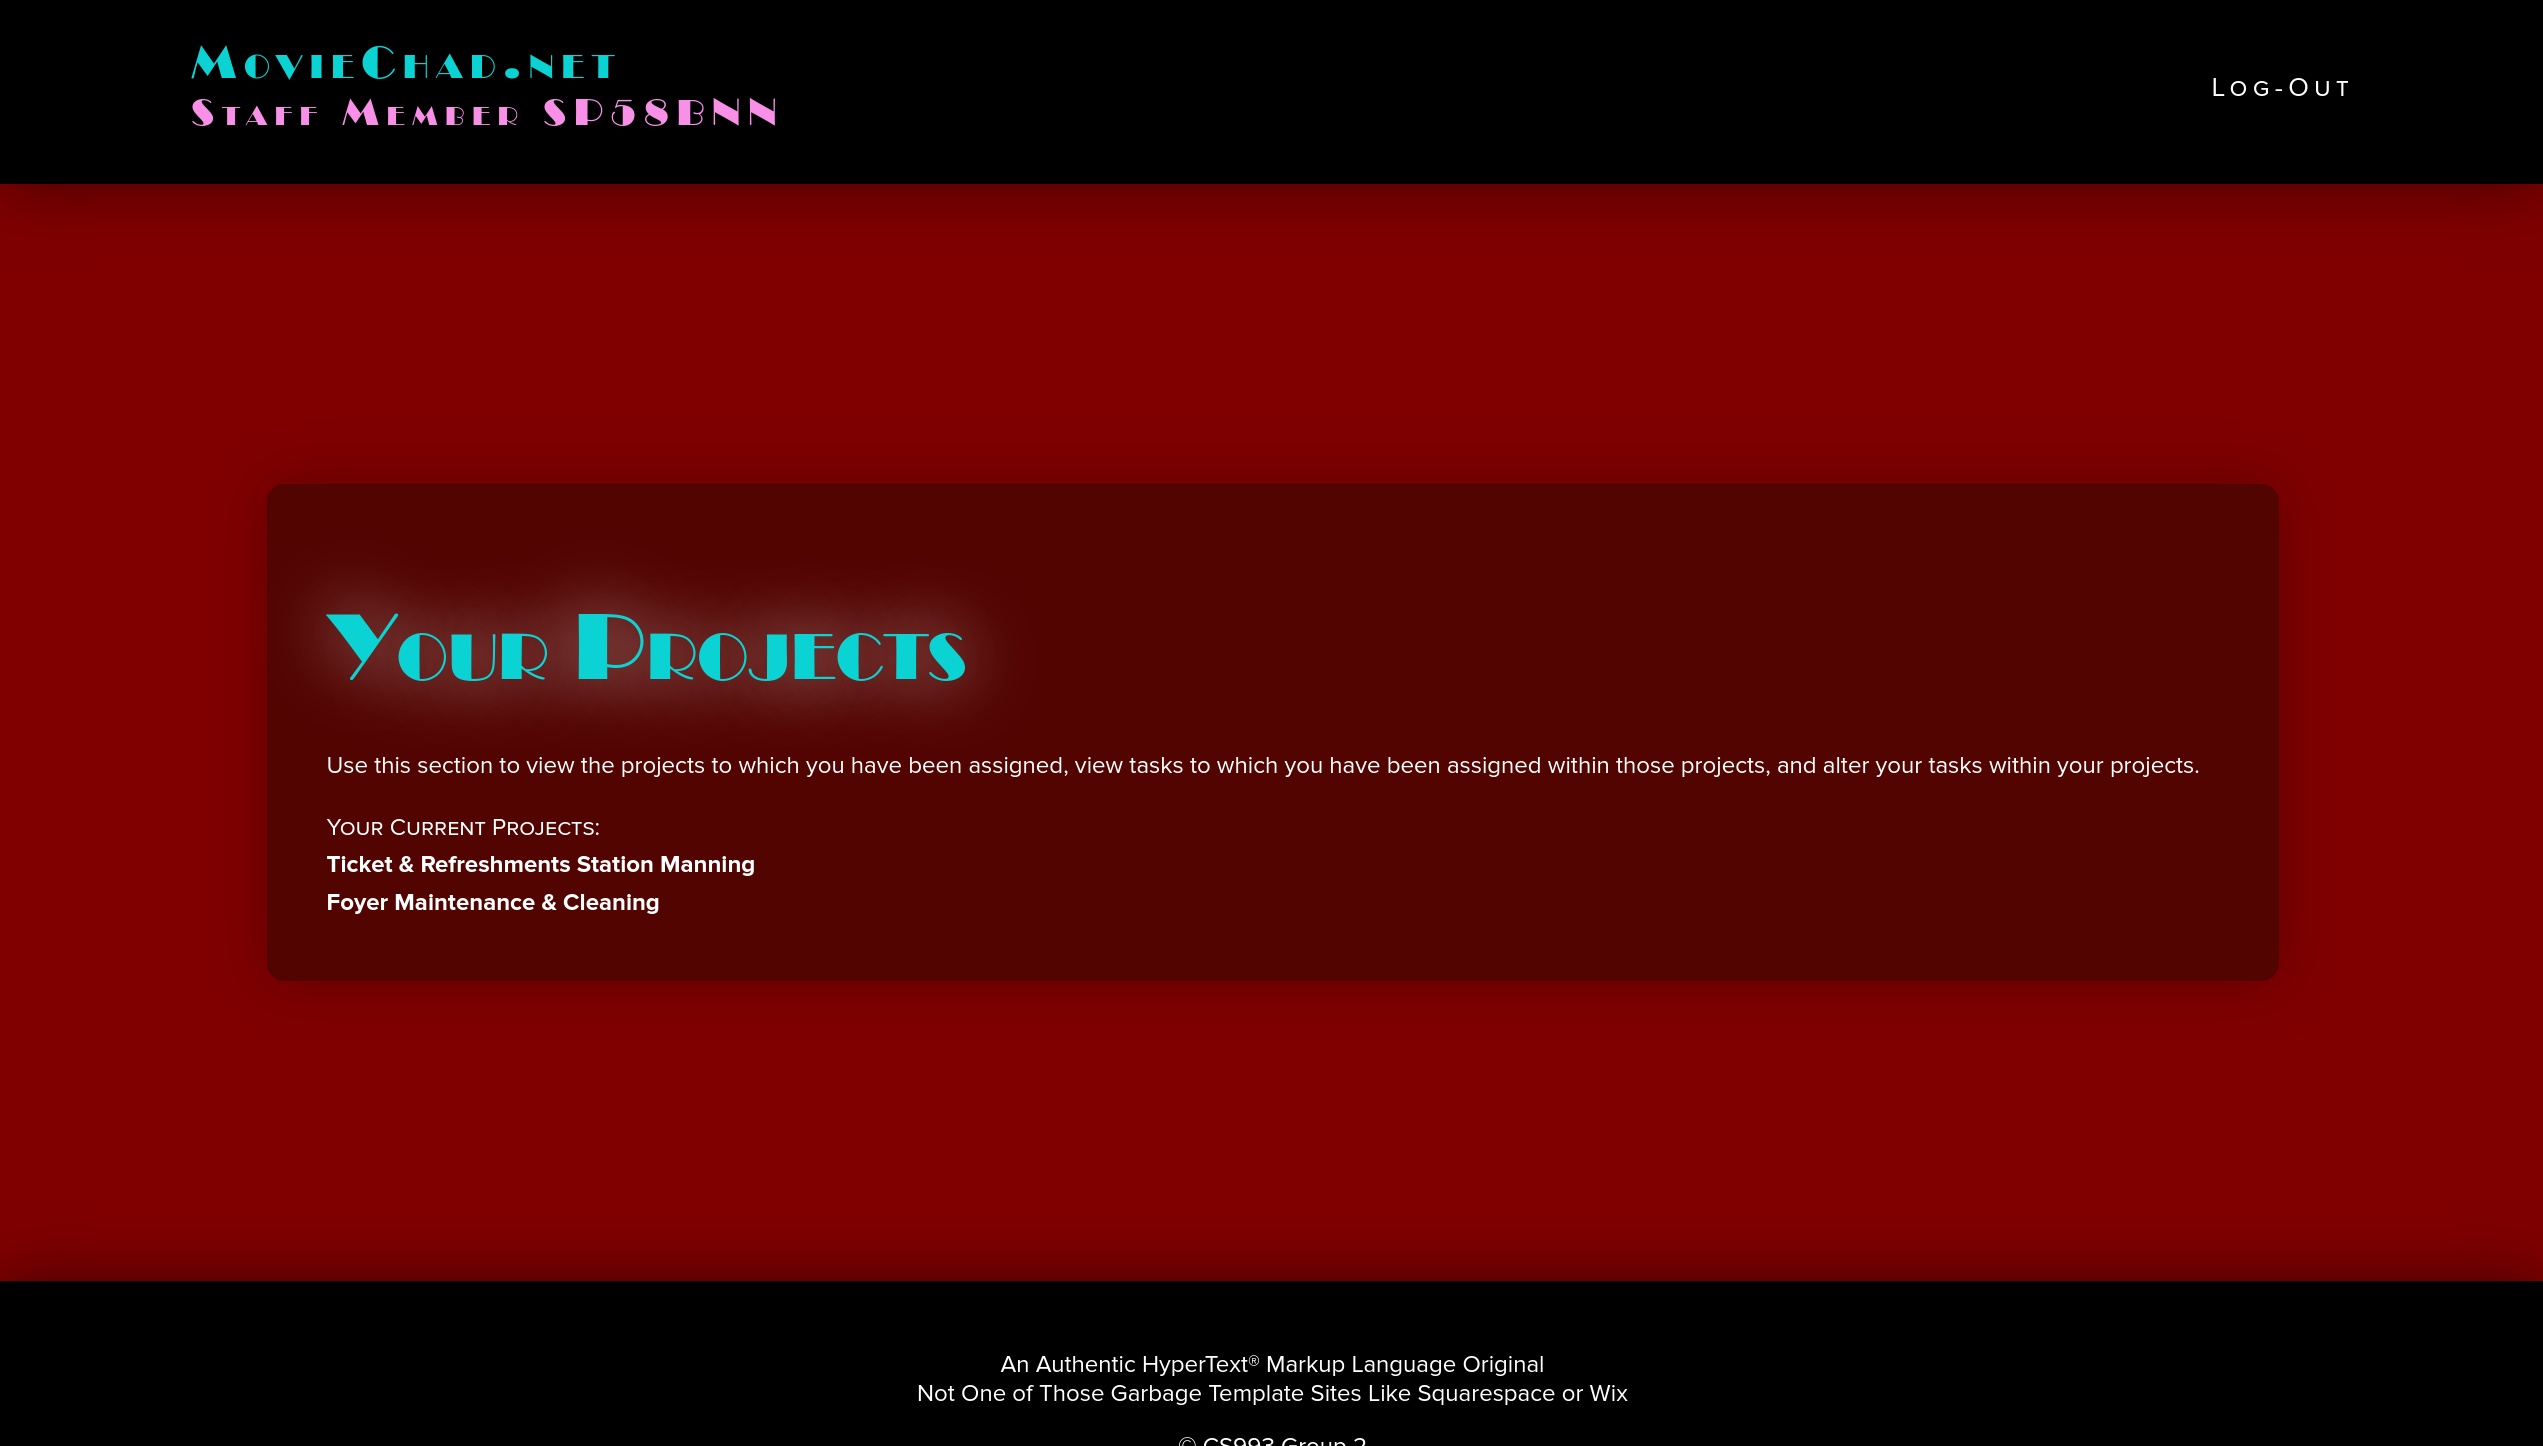
\includegraphics[width=3.25cm,height=2cm]{staff.png} & 
		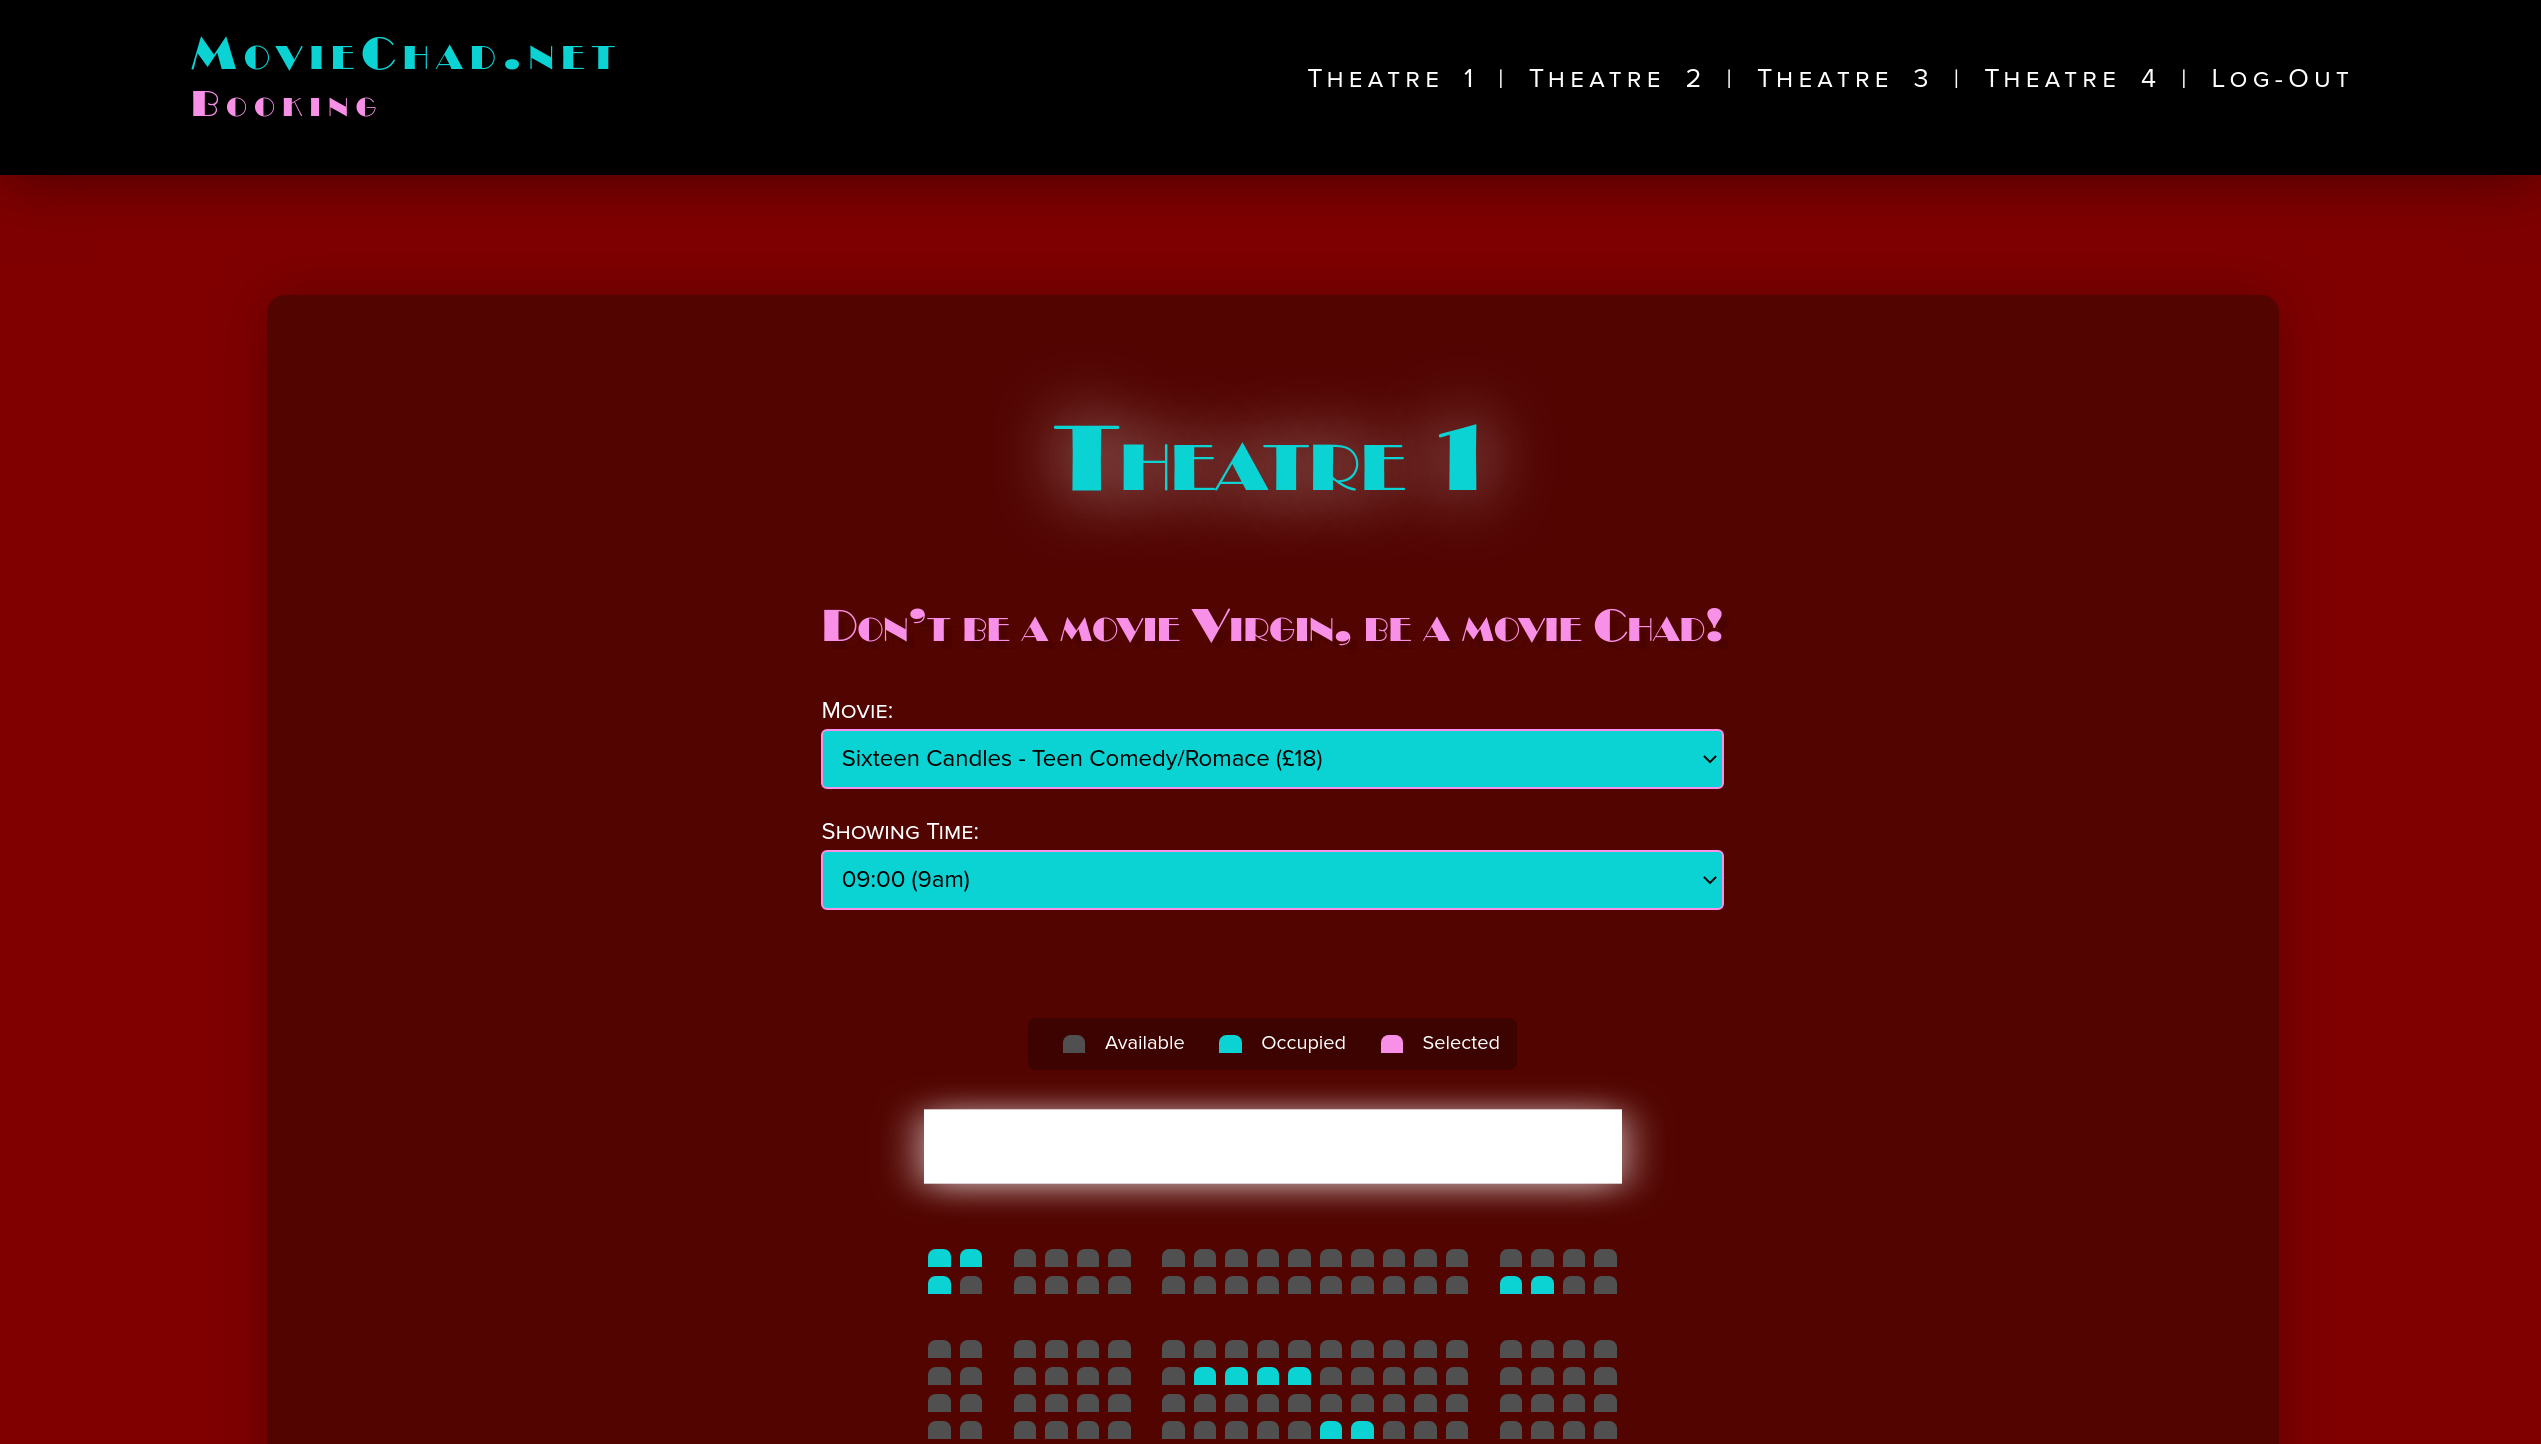
\includegraphics[width=3.25cm,height=2cm]{booker.png}\\
		\textsc{Log-In} & \textsc{Administration} & \textsc{Staff} & \textsc{Booking}\\
	\end{tabular}
	\end{center}

\newpage

	\subsection{Structure}

	\tikzstyle{level 1}=[level distance=1cm, sibling distance=4.5cm]
        \tikzstyle{level 2}=[level distance=1cm, sibling distance=2cm]
        \tikzstyle{level 3}=[level distance=1cm, sibling distance=1.5cm]
        \tikzstyle{level 3}=[level distance=1.5cm, sibling distance=1.25cm]

	\tikzstyle{bag} = [text width=5em, text centered]
        \tikzstyle{end} = [text width=7em, text centered]
	
	{\scriptsize\begin{tikzpicture}
		\node[bag] {Log-In}
			child {
				node[bag] {Administrator}
					child {
						node[end] {Add\\Film}
							child {
								node[end] {Details,\\Theatre,\\Remove Film}
							}
						}
                                	child {
						node[end] {Manage\\Project}
							child {
								node[end] {Staff Shift,\\Element / Time}
							}
						}
                                	child {
						node[end] {Add\\Staff}
							child {
								node[end] {Details,\\Role}
							}
						}
				}
			child {
				node[bag] {Staff}
					child {
						node[end] {View\\Project(s)}
							child {
								node[end] {Details,\\Shift Change,\\Task Comment,\\ New Task}
							}
						}
				}
			child {
				node[bag] {Booker}
					child {
						node[end] {Theatre Booking (1...$N$)}
							child {
								node[end] {Film,\\Showing,\\Seat(s)}
							}
						}
				};
	\end{tikzpicture}}

\newpage

\section{Preliminaries}

	\begin{enumerate}
	\setlength\itemsep{0cm}
		\item Account \textit{projects} and \textit{tasks}
		\item Account user roles \textit{administrator} and \textit{`booker'}
		\item Administrators can assign users to projects and tasks
		\item Any user can book time periods against project or task
		\item Any user can add notes (on what \textbf{was} done), and start/finish time
		\item Administrators must log in as administrators
		\item Users must log in as users
		\item Users can only book projects and tasks they're assigned to
		\item Must scale to mobile devices
	\end{enumerate}

\newpage

	\subsection{Fulfilment}

	\begin{itemize}
	\setlength\itemsep{0cm}
		\item Req. 1: \textit{projects} managed by admins and observed by staff
		\item Req. 1: \textit{tasks} managed by admins and observed / altered by staff
		\item Req. 2: \textit{administrator}: Administrator; \textit{`booker'}: Staff; \textit{`booker'}: Booker
		\item Req. 3: admins can create projects and tasks within, assigning users
		\item Req. 4: staff can request time changes to their assigned shifts on a task 
		\item Req. 4: staff can create their own shift times on new task requests
		\item Req. 5: staff can add notes to a task to which they have been assigned
		\item Req. 6: log-in page has three options: admin, staff, booker
		\item Req. 7: log-in page has three options: admin, staff, booker
		\item Req. 8: staff may only request to add tasks to projects to which they have been assigned
		\item Req. 9: various CSS and JavaScript elements allowing mobile scaling
	\end{itemize}

\end{document}
	%
	% Slide 1:
	%
	% We've designed a web application in the form of a cinema booking system which is slightly different to the original specification. There are three user types implemented to satisfy the criteria. These are administrators, who take the lead role of creating and assigning elements relevant to the cinema context; staff who take the originally specified role of the `booker' in having the ability to be assigned to and self-select project elements relevant to the cinema context; and the additional user: booker, who does not take the brief specified role of a booker and instead takes the simulated role of an actual cinema-goer, meaning they book the viewing of films created, managed and maintained by admins and staff.
	% Note that the booker serves no function to specification requirements however is relevant to the context. The booker is also not generally seen on the industrial side of an application (that is, alongside admin and staff login) however, implementing all users within one log-in system significantly simplifies the project
	% As this is a web application, the interface is written using HTML, CSS and JavaScript, of course not using any bloated IDEs or frameworks; just Bram Moolenar's Vim. Particular CSS and JavaScript elements make this application scalable to mobile devices, in-line with the specification.
	% The rear-end involves various aspects of SQL and the functional use of Python in order to manage user data, requests and inputs.
	%
	% Slide 2:
	%
	% The recursion tree on this slide highlights the structure of the site's hierarchy and some of the basic functions implemented in order to satisfy the specification requirements. This includes the abilities to add films, manage projects and add members of staff as an admin; view and interact with the attributes of projects as a member of staff; and to book film showings as a movie booker.
	%
	% Slide 3:
	%
	% This structure ensures that all of the preliminary specification requirements are met, as outlined here.
	%
